\subsection{Caso de uso 8.1: Modificar vehículos} \label{cu8_1}
\subsubsection{Resumen}
Este caso de uso permite al administrador poder modificar un vehículo
\subsubsection{Descripción}
\begingroup
\setlength{\LTleft}{-10cm plus -1fill}
\setlength{\LTright}{\LTleft}
\begin{center}
  \captionof{table}{\nameref{cu8_1}} \label{tab:cucu8_1_tab}
  \begin{longtable}{| p{3.5cm} | p{11.5cm} |}
        \hline
            \textbf{Versión} &  \\
        \hline 
            \textbf{Autor} & \\
        \hline
           \textbf{Estatus} & \\
        \hline  
            \textbf{Fecha de último estatus} &  31 de marzo de 2017\\
        \hline
      \multicolumn{2}{c |}{\large{Atributos:}} \\
        \hline
          \textbf{Actor}  & Administrador\\
        \hline  
          \textbf{Propósito} & Permite al administrador modificar un vehículo existente \\
        \hline
          \textbf{Disparador} & Al presionar el botón BTN en la vista IU index\\
        \hline  
          \textbf{Entradas} & 
            \begin{itemize}
              \item 
            \end{itemize} \\
        \hline  
          \textbf{Salidas} &  
              \begin{itemize}
                  \item Se mostrarán los datos para que puedan ser actualizados
              \end{itemize} \\
        \hline  
          \textbf{Precondiciones} & 
            \begin{itemize}
                \item \textbf{Interno:} El actor debe ingresar al sistema como administrador
              \end{itemize} \\
        \hline  
          \textbf{Postcondiciones} &  
                \begin{itemize}
                \item \textbf{Interno:} Confirmación de datos actualizados con éxito
              \end{itemize} \\
        \hline
          \textbf{Reglas de negocio} & 
              \begin{itemize}
                  \item {\hyperref[rnr_04]{RNR 04: Campos obligatorios}}
                 \item {\hyperref[rnr_01]{RNE 01: Cuenta válida}}
              \end{itemize} \\
        \hline
          \textbf{Mensajes} & 
              \begin{itemize}
                 \item {\hyperref[msje_01]{MSJE 01: Datos inválidos}}
              \end{itemize} \\
        \hline
          \textbf{Tipo} & \\
        \hline      
  \end{longtable}
\end{center}
\endgroup

\subsubsection{Trayectorias del caso de uso}
\textbf{Trayectoria principal}
\begin{enumerate}
  \item {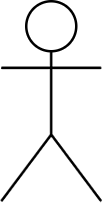
\includegraphics[scale=.1]{Capitulo3/img/actor.png} Ingresa el administrador al portal web mediante una dirección eletrónica.}
  \item {
\includegraphics[scale=.05]{Capitulo3/img/proceso.png} Se muestra la vista IU Index para el administrador.}
  \item {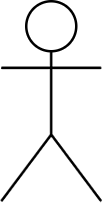
\includegraphics[scale=.1]{Capitulo3/img/actor.png} Presiona el botón de Iniciar sesión.}
  \item {
\includegraphics[scale=.05]{Capitulo3/img/proceso.png} Se muestra la vista IU Index.}
  \item {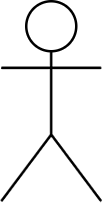
\includegraphics[scale=.1]{Capitulo3/img/actor.png} Selecciona el administrador el botón \textit{Consultar catálogo}}
  \item {
\includegraphics[scale=.05]{Capitulo3/img/proceso.png} Se muestra la vista IU Catálogo.}
  \item {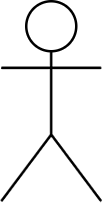
\includegraphics[scale=.1]{Capitulo3/img/actor.png} Selecciona el administrador el botón \textit{Modificar vehículo}}
  \item {
\includegraphics[scale=.05]{Capitulo3/img/proceso.png} Se muestra la IU vehículo }
  \item {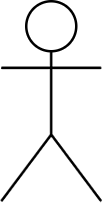
\includegraphics[scale=.1]{Capitulo3/img/actor.png} Selecciona el vehículo a actualizar }
  \item {
\includegraphics[scale=.05]{Capitulo3/img/proceso.png} Se muestra la IU vehículo datos }
  \item {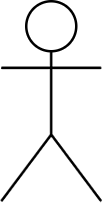
\includegraphics[scale=.1]{Capitulo3/img/actor.png} Actualiza los datos necesarios }
  \item {
\includegraphics[scale=.05]{Capitulo3/img/proceso.png} Se confirma la actualización de datos }
    \textit{Fin de caso de uso} \\  
\end{enumerate}


\textbf{Trayectoria alternativa} \phantomsection\label{cu_ta_} \\
\textbf{Condición:} \\
 \begin{enumerate}[label=\arabic*]
    \item {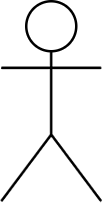
\includegraphics[scale=.1]{Capitulo3/img/actor.png} }
    \item {
\includegraphics[scale=.05]{Capitulo3/img/proceso.png}}
    \item {Continua en el paso 4 de la trayectoria principal.} \\
    \textit{Fin de trayectoria} \\
\end{enumerate}


\subsubsection{Puntos de extensión}
\noindent \textbf{Causa de la extensión:} El actor, de tipo administrador, oprimió el botón \textit{Modificar vehículo} \\
\textbf{Región de la trayectoria:} \hyperref[cu_ta_]{Trayectoria alternativa } \\
\textbf{Extiende a:} \hyperref[cu7]{CU 7 Consultar catalogos}
